
\chapter{Bubble Imaging Methods} \label{related_work}
 

This chapter briefly discusses two similar bubble measurement techniques that aim to estimate bubble concentrations in water. The first is a master's thesis by \citet{Leonie}, where a bright field method was used in a wind wave facility, so that bubbles appeared as dark circles on camera. The second is a field measurement technique \citep{Al-Lashi2016}, where bubbles were artificially lit from below, yielding similar images to the ones discussed in this thesis, and the third one is the method proposed by this work. 

\section{Bright field method}
	As an improved method from \citet{MischlerDiss}, \citet{Leonie} uses a bright field method as shown in figure \ref{fig:bright_field}. Bubbles in this experimental setup are backlit, so that they appear completely dark except for one spot in the center (see section  \ref{bubble_physics}). Note the need to use a lens shift adapter because the incoming rays are not parallel. 
	
		\begin{figure}
			\centering
			\begin{subfigure}[t]{0.55\textwidth}
				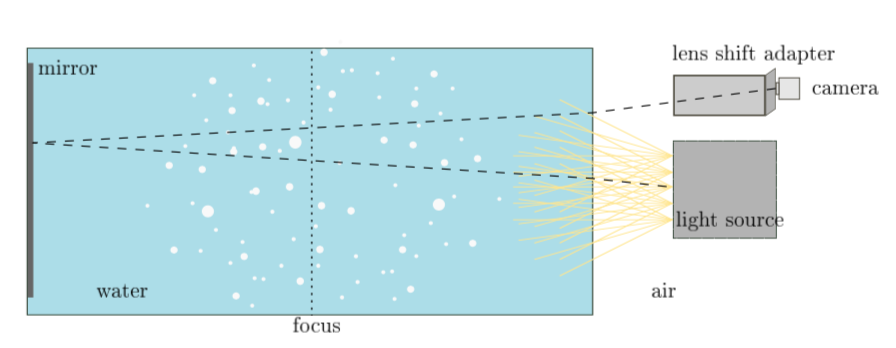
\includegraphics[scale=.4]{images/bright_field_method.png}
				\caption{Experimental setup of a light field method at Aeolotron facility}
			\end{subfigure}
			
			\begin{subfigure}[t]{0.3\textwidth}
				\centering
				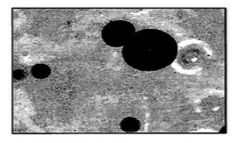
\includegraphics[scale=0.5]{images/bright_field_result.png}
				\caption{Sample result image}
			\end{subfigure}%
			\begin{subfigure}[t]{0.3\textwidth}
				\centering
				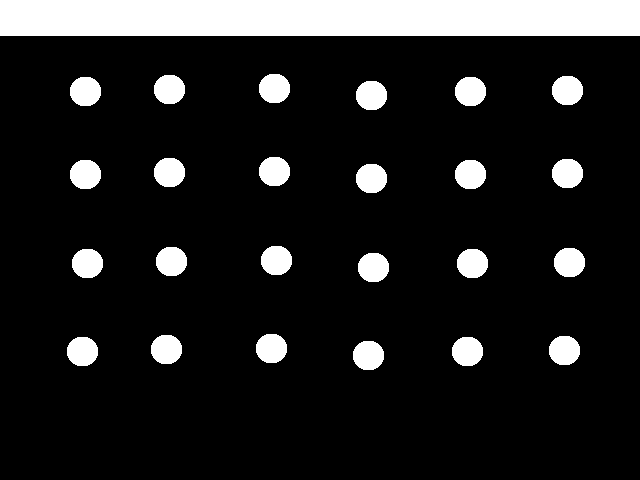
\includegraphics[scale=0.15]{images/bright_field_calibration_target.png}
				\caption{calibration target}
				\label{subfig:calib_target}
			\end{subfigure}
			
			\caption{In the bright field method, bubbles are back-lit. Bubbles scatter the incoming light away such that they appear as dark disks. }
			\label{fig:bright_field}
		\end{figure}		
	
	Depth of field calibration was based on the edges between bubbles and background. The higher the edge's magnitude, the closer the bubble is to the focus plane. A calibration target made of hollow circles was used to calibrate the depth of field (figure \ref{subfig:calib_target}). 
	
	The images obtained by this method are arguably the most important advantage of this technique, since it reduces bubbles to simple circles, making them relatively easy to detect, whereas our algorithms need to recognize significantly more complex patterns than mere circles.
	 In contrast to our method however, the bright field technique constrains how close the camera can get to the water surface. Also, \citet{Leonie} does not define a criterion that measures how well the circle detection algorithm performs, so the assumption is that precision is close to perfect, which introduces an error to bubble concentration measurement that was essentially neglected. 
	 Nevertheless, this work was very important for the newly developed method in this work, because it offered an estimation of boundary conditions, such as the largest possible bubble radius and the largest possible bubble concentration, which were important to determine the different hyperparameters of the proposed algorithms in this thesis and therefore contributing to the accuracy of the algorithms. 
	
	
\section{Bubble optical imaging instrument}
	This technique is a field method that submerges an optical imaging instrument underwater and illuminates a thin slice	of water of volume from above and below. 
	This method is particularly interesting because it produces images similar to our own. The
	However, applying the algorithm from this paper did not yield good results. This is most likely due to the fact that our method does not illuminate the bubbles from above, making the bubble's circular shape not easily detectable with a simple Hough transform \citep{Hough1972}.


\section{Proposed Method}
The proposed method in this work aims to measure bubbles that are as close to the water surface as possible, and to develop robust algorithms that can reliably detect bubbles, estimate their radii and their depths (i.e.\ distance to focal plane). In particular, the proposed method should perform well for high and low bubble concentrations. 
The principle behind this method is to light air bubbles in a water tank from below, and position the camera on the side of the water tank. The reflected light on the lower edge of bubbles is then captured by the camera. 

The main drawback of this method, however, is that small bubbles with less than 6 to 8\,px in diameter can not be detected. 



















